\documentclass{standalone}
\usepackage{pgfplots}
\usepackage{sansmath}
\pgfplotsset{compat=1.16}
\definecolor{bg}{HTML}{D8D8D8}
\definecolor{Display}{HTML}{1F77B4}
\definecolor{LowerExp}{HTML}{FF7F0E}
\definecolor{dtoa}{HTML}{2CA02C}
\definecolor{ryu}{HTML}{9467BD}
\definecolor{lexical}{HTML}{D62728}
\definecolor{teju}{HTML}{9C564B}
\definecolor{zmij}{HTML}{E377C2}
\tikzset{
  on layer/.code={
    \pgfonlayer{#1}\begingroup
    \aftergroup\endpgfonlayer
    \aftergroup\endgroup
  },
}
\pgfplotsset{
  every axis/.append style={
    x=12pt,
    height=3.5in,
    xmin=0.5,
    ymin=0,
    ymax=87,
    xtick pos=bottom,
    xtick distance=5,
    ytick distance=10,
    xticklabel shift=-1pt,
    tick label style={font=\sansmath\sffamily},
    every axis label={font=\sansmath\sffamily},
    label style={font=\sansmath\sffamily},
    ymajorgrids=true,
    major grid style={line width=0.8pt,draw=gray!55},
    axis background/.style={fill=bg},
  },
  every axis plot/.append style={
    line width=0.8pt,
    mark=*,
    forget plot,
  },
  area legend/.style={
    legend image code/.code={
      \draw[#1] (0pt,0.3pt) rectangle (0.9em,1.4ex);
    },
  },
  highlight/.style={
    preaction={
      on layer=pre main,
      line width=6pt,
      opacity=0.5,
      line cap=round,
      line join=round,
      yellow,
    },
  },
}
\begin{document}
\pagecolor{white}
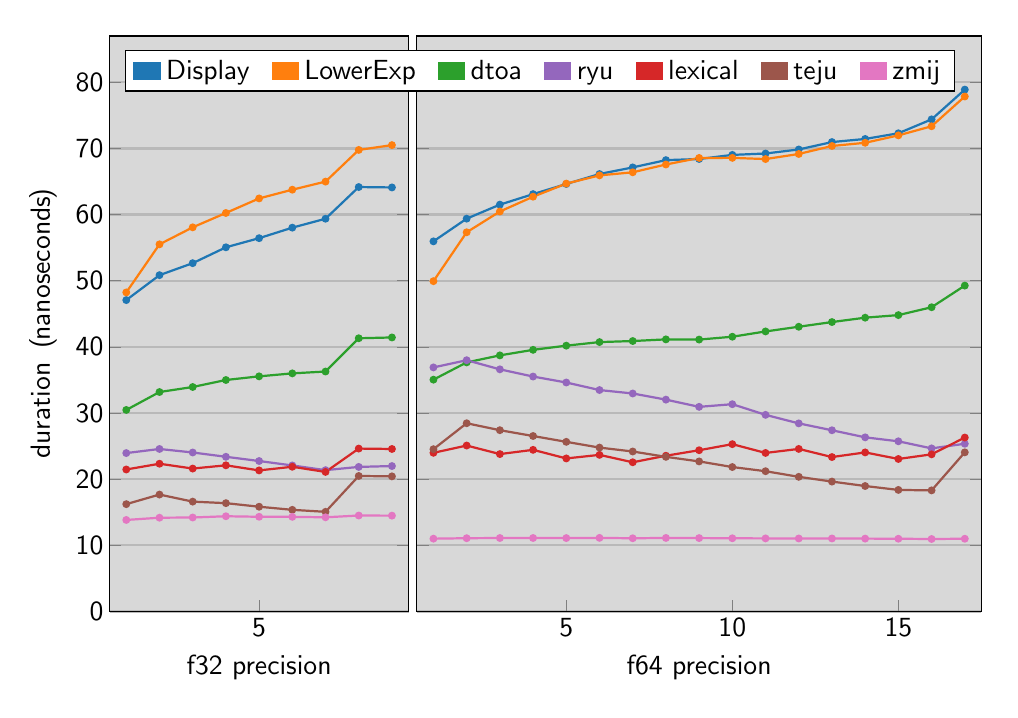
\begin{tikzpicture}[
  every mark/.append style={mark size=1pt},
]
\begin{axis}[
  name=f32,
  xmax=9.5,
  xlabel={f32 precision},
  ylabel={duration\enskip(\kern-1pt nanoseconds\kern-1pt)},
  yticklabel shift=-1.25pt,
  set layers,
  legend style={
    anchor=north west,
    at={(0.05,0.975)},
    font=\sansmath\sffamily,
    /tikz/every even column/.append style={column sep=6pt},
    nodes={anchor=base, inner ysep=0.5pt},
    execute at begin node={\rule{0pt}{8pt}},
  },
  legend cell align=left,
  legend columns=-1,
]
  \addlegendentry{Display}
  \addlegendimage{color=Display, fill, area legend}
  \addplot[color=Display] coordinates {
    (1, 47.07)
    (2, 50.84)
    (3, 52.65)
    (4, 55.05)
    (5, 56.43)
    (6, 58.02)
    (7, 59.37)
    (8, 64.16)
    (9, 64.10)
  };
  \addlegendentry{LowerExp}
  \addlegendimage{color=LowerExp, fill, area legend}
  \addplot[color=LowerExp] coordinates {
    (1, 48.23)
    (2, 55.50)
    (3, 58.07)
    (4, 60.24)
    (5, 62.44)
    (6, 63.76)
    (7, 64.98)
    (8, 69.77)
    (9, 70.50)
  };
  \addlegendentry{dtoa}
  \addlegendimage{color=dtoa, fill, area legend}
  \addplot[color=dtoa] coordinates {
    (1, 30.46)
    (2, 33.17)
    (3, 33.93)
    (4, 34.99)
    (5, 35.54)
    (6, 35.99)
    (7, 36.27)
    (8, 41.30)
    (9, 41.42)
  };
  \addlegendentry{ryu}
  \addlegendimage{color=ryu, fill, area legend}
  \addplot[color=ryu] coordinates {
    (1, 23.94)
    (2, 24.56)
    (3, 24.03)
    (4, 23.38)
    (5, 22.74)
    (6, 22.07)
    (7, 21.36)
    (8, 21.85)
    (9, 21.98)
  };
  \addlegendentry{lexical}
  \addlegendimage{color=lexical, fill, area legend}
  \addplot[color=lexical] coordinates {
    (1, 21.46)
    (2, 22.33)
    (3, 21.60)
    (4, 22.09)
    (5, 21.32)
    (6, 21.87)
    (7, 21.09)
    (8, 24.62)
    (9, 24.56)
  };
  \addlegendentry{teju}
  \addlegendimage{color=teju, fill, area legend}
  \addplot[color=teju] coordinates {
    (1, 16.22)
    (2, 17.67)
    (3, 16.60)
    (4, 16.37)
    (5, 15.83)
    (6, 15.36)
    (7, 15.06)
    (8, 20.48)
    (9, 20.42)
  };
  \addlegendentry{zmij}
  \addlegendimage{color=zmij, fill, area legend}
  \addplot[color=zmij] coordinates {
    (1, 13.83)
    (2, 14.17)
    (3, 14.20)
    (4, 14.39)
    (5, 14.31)
    (6, 14.30)
    (7, 14.23)
    (8, 14.50)
    (9, 14.48)
  };
\end{axis}
\begin{axis}[
  name=f64,
  at=(f32.east),
  anchor=west,
  xshift=3pt,
  xmax=17.5,
  xlabel={f64 precision},
  yticklabel=\empty,
  set layers,
]
  \addplot[color=Display] coordinates {
    (1, 55.95)
    (2, 59.38)
    (3, 61.50)
    (4, 63.09)
    (5, 64.62)
    (6, 66.13)
    (7, 67.13)
    (8, 68.23)
    (9, 68.40)
    (10, 69.02)
    (11, 69.23)
    (12, 69.84)
    (13, 70.96)
    (14, 71.43)
    (15, 72.29)
    (16, 74.39)
    (17, 78.89)
  };
  \addplot[color=LowerExp] coordinates {
    (1, 49.93)
    (2, 57.32)
    (3, 60.46)
    (4, 62.70)
    (5, 64.68)
    (6, 65.92)
    (7, 66.39)
    (8, 67.57)
    (9, 68.56)
    (10, 68.57)
    (11, 68.39)
    (12, 69.16)
    (13, 70.37)
    (14, 70.85)
    (15, 71.97)
    (16, 73.35)
    (17, 77.85)
  };
  \addplot[color=dtoa] coordinates {
    (1, 35.04)
    (2, 37.65)
    (3, 38.71)
    (4, 39.55)
    (5, 40.18)
    (6, 40.72)
    (7, 40.88)
    (8, 41.13)
    (9, 41.10)
    (10, 41.53)
    (11, 42.33)
    (12, 43.04)
    (13, 43.75)
    (14, 44.41)
    (15, 44.80)
    (16, 45.99)
    (17, 49.26)
  };
  \addplot[color=ryu] coordinates {
    (1, 36.89)
    (2, 37.98)
    (3, 36.60)
    (4, 35.51)
    (5, 34.61)
    (6, 33.47)
    (7, 32.95)
    (8, 32.02)
    (9, 30.93)
    (10, 31.33)
    (11, 29.72)
    (12, 28.43)
    (13, 27.39)
    (14, 26.32)
    (15, 25.72)
    (16, 24.65)
    (17, 25.35)
  };
  \addplot[color=lexical] coordinates {
    (1, 23.98)
    (2, 25.08)
    (3, 23.79)
    (4, 24.43)
    (5, 23.13)
    (6, 23.67)
    (7, 22.55)
    (8, 23.54)
    (9, 24.37)
    (10, 25.29)
    (11, 23.96)
    (12, 24.57)
    (13, 23.34)
    (14, 24.04)
    (15, 23.05)
    (16, 23.75)
    (17, 26.29)
  };
  \addplot[color=teju] coordinates {
    (1, 24.53)
    (2, 28.45)
    (3, 27.40)
    (4, 26.52)
    (5, 25.64)
    (6, 24.77)
    (7, 24.18)
    (8, 23.37)
    (9, 22.68)
    (10, 21.83)
    (11, 21.20)
    (12, 20.35)
    (13, 19.63)
    (14, 18.96)
    (15, 18.37)
    (16, 18.30)
    (17, 24.05)
  };
  \addplot[color=zmij] coordinates {
    (1, 11.00)
    (2, 11.07)
    (3, 11.10)
    (4, 11.10)
    (5, 11.09)
    (6, 11.12)
    (7, 11.06)
    (8, 11.11)
    (9, 11.09)
    (10, 11.06)
    (11, 11.04)
    (12, 11.03)
    (13, 11.03)
    (14, 11.01)
    (15, 10.99)
    (16, 10.95)
    (17, 10.99)
  };
\end{axis}
\pgfresetboundingbox\path
  (f32.south west) -- ++(-0.41in,-0.39in)
  rectangle (f64.north east) -- ++(6pt,3pt);
\end{tikzpicture}
\end{document}
